% ======================================================================================================
% NOTES, TODOS
% ======================================================================================================
\subsection{Search Result and Bibliometric Analysis}

After completing the selection process, which involved applying inclusion and exclusion criteria and eliminating duplicate studies, 67 research papers were considered eligible for further review and analysis. The accompanying pie chart (see Figure \ref{fig:archive-itemtype}) reveals that IEEE was the primary publisher of the selected papers, accounting for 44 of them. SpringerLink was the second largest contributor, with 12 publications, while Elsevier (5), ACM (4), and MDPI (2) each account for the lowest contribution of publications. The second right side of the pie chart \ref{fig:archive-itemtype} also demonstrates that the majority of the selected papers were sourced from Web of Science and Scopus, followed by IEEE and SpringerLink. It is important to note how the selected papers are distributed in terms of publishing kinds. Of these papers, i.e. 67\% -or 45-were published as conference papers, whereas the remaining 32\% -or 22-were in the form of journal articles.




% Cluster one encompasses terms related to 4G technology, machine learning, real-time security analysis, security frameworks, access control, and automation, highlighting the importance of incorporating advanced technologies in the field of security and access control automation. This cluster also suggests a growing emphasis on real-time security analysis to ensure quick identification and response to potential threats.

% Cluster two comprises keywords such as cybersecurity, data models, digital twin, internet of things, privacy, prototypes, safety, and cloud computing. The inclusion of terms such as privacy, prototypes, and safety in this cluster indicates a growing concern for the protection of sensitive information and the security of digital representations of physical systems. 

% The third cluster encompasses terms such as those related to the automotive industry, availability, blockchain, industry 4.0, industrial control systems, system life cycles, intelligent control, software, and tools. This cluster suggests a growing emphasis on the use of blockchain technology for secure data management in the automotive industry for data sharing. 

% The fourth cluster is comprised of analytical models, anomaly detection, cyber-attacks, monitoring, resilience, critical infrastructure, integrated circuits, and physical systems. This cluster shows the association of identification and mitigation of potential security threats through the use of analytical models to detect anomalies to increase the resilience of critical infrastructure.

% The final cluster includes terms such as cyber-physical systems, e-learning, embedded systems, predictive models, and smart grids. This cluster highlight the importance of training and education to promote the secure use of cyber-physical system such as smart grids.

% This is some text with a \coloredcircle{yellow} small circle in red color next to it \coloredcircle{#00ff00}

% \begin{figure}
% \includesvg[width=0.5\textwidth]{images/svg/databases.svg}
% \includesvg[width=0.5\textwidth]{images/svg/itemtype.svg}
% \svgcaption{This is the label for the SVG image.}
% \label{fig:image}
% \end{figure}

\begin{figure}[H]    
    % \centring
    \begin{subfigure}[b]{0.48\textwidth}
        \includegraphics[width=\textwidth]{images/newimages/pie-paper-publisher.png}
        % \includesvg[width=\textwidth]{images/svg/databases.svg}
        \caption{Number of Selected Papers Per publisher.}
    \end{subfigure}
    \begin{subfigure}[b]{0.45\textwidth}
        \includegraphics[width=\textwidth]{images/newimages/pie-paper-source.png}
        % \includesvg[width=\textwidth]{images/svg/itemtype.svg}
        \caption{Number of Selected Papers Per Pource.}
    \end{subfigure}
    \caption{An Analysis of Paper Distribution Based on Source and Publisher.}
    \label{fig:archive-itemtype}
\end{figure}
 
Analysis of the distribution of selected papers based on publication year revealed that the majority of articles were published in 2022 and 2021 (see Figure \ref{fig:bar-chart-yaer}). Furthermore, the bar chart illustrates a general upward trend in the number of publications addressing security concerns for industries utilising Digital Twin and (I)IoT applications.  This trend indicates a growing interest and concern among researchers in the Digital Twin and (I)IoT security field and highlights the relevance of this systematic literature review.

Note that the data in the figure of search results obtained on May 14th, 2023 contain only 6 papers for the year 2023. Since this number covers less than half a year and considering the trend of published articles from the last 5 years, we expect a further increase in the number of papers by the end of 2023.

\begin{figure}[H]    
    \caption{Yearly Publication Statistics: Investigating the Number of Papers Published}
    % \includesvg[width=0.9\textwidth]{images/svg/pub_year_white_bg.svg}
    \includegraphics[width=\textwidth]{images/newimages/barchart-year.png}
    \caption{Distribution of Papers Published Per Year}
    \label{fig:bar-chart-yaer}
\end{figure}

\subsubsection*{Keyword Frequency Analysis}
To gain a deeper understanding of the trending topics within the 67 selected papers published between 2018 and 2023, a frequency analysis of keywords was conducted. This analysis was performed by extracting keywords that appeared more than three times in the keyword sections of the articles using the VOSviewer \footnote{\url{https://www.vosviewer.com/} A tool for visualizing bibliometric network including the occurrence of keywords, coauthorship relationship.} tool. 

Further filtering and sensitization were applied to create a shortlist of keywords using a thesaurus text file (a text file used by VOSviewer with one column for keywords and another column for replacing words). Keywords which have similar meanings with different spellings and variations were merged. For instance, we replaced "artificial intelligence" and "deep learning" with "machine learning", and "intrusion detection" with anomaly detection. We also replaced the occurrence of "security" with "cybersecurity". We combined "control systems" under the term "industrial control system". "Smart grid" and "power grid" are considered similar concepts. Additionally, we have replaced the term "real-time" with "real-time system". We considered "emulation" and "simulation" as related concepts hence we used the "simulation" keyword as a representative for "emulation". 

The resulting frequency analysis of keywords, illustrated in Figure \ref{fig:alluvial-key}, provides insight into the key themes and concepts that are prevalent in the research topic of Digital Twin and cybersecurity. In addition, this analysis can help guide future research by identifying areas where there is a need for further investigation and providing a sense of the current state of the field.

\begin{figure}[H]
    % \includesvg[width=0.9\textwidth]{images/svg/key_buble.svg}
    % 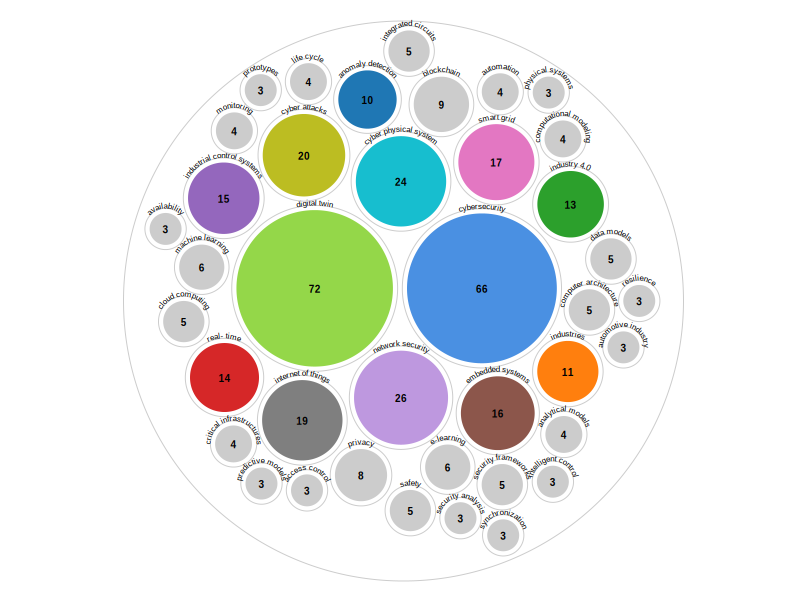
\includegraphics[width=\textwidth]{images/svg/key_buble.png}
    \includegraphics[width=1\linewidth]{images/rt/keywordoccurence.png}
    \caption{Frequency of Keywords from Keyword Section of 67 Papers}
    \label{fig:alluvial-key}
\end{figure}


'digital twin' with 55 occurrences indicates the centrality of this concept in this review. 'cybersecurity' is the second most frequently mentioned word, indicating the selected papers focus on using Digital Twin to provide security services. 'iot' is the third a frequent mention word with 19 times mention.   This highlights the significant role of this enabling technology in sending and receiving data to and from the Digital Twin environment. 

This analysis identified several key enabling technologies, namely 'blockchain(9),' 'machine learning(8)' 'cloud computing(4)' and 'analytics(3)'. These technologies are the main driving force of Digital Twin to be used as a security tool. 

Our frequency analysis also revealed the prevalent adoption of Digital Twin within Industry 4.0, as evidenced by terms such as 'cyber-physical systems(8)', 'smart grid(7)', and 'industrial control systems(6)'. These industry sectors highlight the integration and utilization of Digital Twin in critical infrastructure, indicating its role in providing various services including security-related functions. 


The main security and non-security functions of Digital Twin identified from the analysis were 'anomaly detection(7)', 'network security(6)', and 'simulation(6)'. This indicates the growing interest in leveraging Digital Twin frameworks for proactive security measures (anomaly detection), monitoring and detecting security problems in interconnected networks and utilizing simulation techniques for testing security measures before they are deployed to real operation environments to avoid accidental failure. 

\subsubsection*{Keyword Co-relationship Network}
In order to gain further insights into the evolution of research in the field of Digital Twin and cybersecurity, a keyword co-relationship network analysis was extracted from the VOSviewer tool. 

This analysis aimed to identify clusters of related items and visualise the relationships between keywords over time. The results of this analysis revealed that in the early days of research on Digital Twin, keywords such as "computational modelling", "embedded system", "situational awareness", "safety", and "simulation" were frequently mentioned, which suggests that the primary focus of the research at that time was on utilising Digital Twin as a visual aiding tool. 

On the other hand, more recent research was characterized by the frequent mention of emerging technologies such as "blockchain," "machine learning," "e-learning" "5G," and "emulation" This indicates that the development of Digital Twin has shifted towards utilising these technologies and augmenting Digital Twin to provide more service other than used as a model.



\begin{figure}[H]
    % \centering    
    \includegraphics[width=\textwidth, center]{images/newimages/vosviewer-2oc.png}
    % \includesvg[width=\textwidth]{images/new}
    % \includesvg[inkscapelatex=false,width=0.95\columnwidth]{images/key_belt.svg}
    \caption{keyword co-relationship from VOSviewer}
    \label{fig:co-occurrence-vosv}
\end{figure}

The analysis of the co-occurrence of keywords in the selected articles, as represented in Figure \ref{fig:co-occurrence-vosv}, identified eight clusters. As defined by the VOSviewer documentation, these clusters are groups of terms that exhibit a high degree of relatedness. 


\textit{Cluster One:}
This cluster focuses on various aspects related to the industrial and digital domains. It includes topics such as authentication, autonomous vehicles, cloud computing, costs, digital twin, industrial Internet of things (IIoT), microgrids, real-time systems resilience, and smart manufacturing. The common theme in this cluster appears to be the integration of digital technologies in industrial settings, emphasizing security, efficiency, and advanced manufacturing processes.

\textit{Cluster Two:}
This cluster revolves around computer-related topics, computational modelling, computer architecture, and embedded systems. It also includes subjects like cyber-physical systems, industry 4.0, network security, situational awareness, and smart grids. The primary focus here seems to be the intersection of computer science and engineering, with an emphasis on the integration of smart technologies into physical systems and networks.

\textit{Cluster Three:}
Cluster three is centered around security and privacy concerns in the digital landscape. It encompasses topics such as blockchain, cyber Digital Twin, cybersecurity, data privacy, safety, smart cities, smart contracts, soft sensors, and traffic control. The key theme here is the exploration of secure and privacy-preserving solutions in digital ecosystems, including blockchain technology and data protection measures.

\textit{Cluster Four:}
This cluster focuses on topics related to access control, automation, data security, and smart homes within the Internet of Things (IoT) context. The cluster includes items such as access control, automation, data security emulation, and IoT smart homes. The primary theme revolves around securing and managing access to IoT devices and systems, as well as exploring automation and smart home technologies.

\textit{Cluster Five:}
Cluster five centers on industrial control systems and security. It includes topics such as industrial control systems, integrated circuits, intelligent control, intrusion detection, machine learning, predictive models, and security-by-design. The focus here is on ensuring the security and reliability of industrial control systems, incorporating intelligent control algorithms, and leveraging machine learning for intrusion detection and predictive maintenance.

\textit{Cluster Six:}
This cluster encompasses topics related to communication networks and security frameworks. It includes items such as 5G, cyber range, industries, pipelines, security framework, security operation center, and wireless communication. The primary theme is the exploration of cyber range for training employees in sectors such as 5g network and security operation center. 



\textit{Cluster Seven:}
Cluster seven revolves around anomaly detection, cyber-physical systems, deep learning, monitoring, and SCADA systems. The focus here is on leveraging advanced techniques such as deep learning and anomaly detection for monitoring and securing cyber-physical systems, particularly in the context of SCADA systems.

\textit{Cluster Eight:}
Cluster eight is centered around analytical models, simulation, and testing. The focus is on the development and application of analytical models and simulation techniques for testing and evaluating various systems or scenarios.